\section{Introduction}
\begin{frame}
    \sectionpage
\end{frame}

\begin{frame}{Quantum Computing 101}
    \begin{block}{What is a quantum computer?}
        A device that performs computations by exploiting the properties of quantum states:
        \begin{itemize}
            \item \textbf{Superposition}: the combination of quantum states is a quantum state
            \item \textbf{Entanglement}: the quantum state of a particle depends on the state of other particles
            %\item \textbf{Interference}
        \end{itemize}
    \end{block}
\end{frame}

\begin{frame}{Quantum Computing 101}
    \begin{columns}[t, totalwidth=1.02\textwidth]
        \begin{column}{0.45\linewidth}
            \begin{block}{What is a qubit?}
                    \begin{itemize}
                        \item The basic unit of quantum information
                        \item Represented as a quantum superposition of two basis states
                    \end{itemize}
                    \begin{equation*}
                        |\psi \rangle = \alpha | 0 \rangle + \beta | 1 \rangle
                    \end{equation*}
            \end{block} 
        \end{column}
        \begin{column}{0.45\linewidth}
            \begin{figure}
                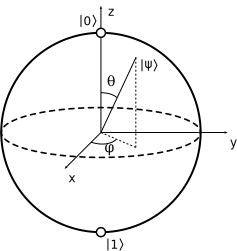
\includegraphics[scale=0.4]{images/Bloch_sphere.png}
            \end{figure}
        \end{column}
    \end{columns}
\end{frame}

\begin{frame}{Classic computers \textit{vs} classic cryptography}
    \begin{block}{Symmetric cryptosystems}
        \textbf{Key enumeration}: perform an exhaustive search on the whole keyspace, $\mathcal{O}(n)$ time
    \end{block}
    \begin{block}{Asymmetric cryptosystems}
        \textbf{General number field sieve}: factor a composite number $n$ is $\mathcal{O}(e^{1.9(\log{n})^{1/3})(\log{\log{n}})^{2/3}})$ (subexponential) time
    \end{block}
\end{frame}

\begin{frame}{Quantum computers \textit{vs} classic cryptography}
    \begin{block}{Symmetric cryptosystems}
        \textbf{Grover's algorithm}: search in a database of $n$ elements in $\mathcal{O}(n^{1/2})$ time and $\mathcal{O}(\log n)$ space
    \end{block}
    \begin{block}{Asymmetric cryptosystems}
        \textbf{Shor's algorithm}: factor a composite number $n$, on a quantum computer, in $\mathcal{O}((\log{n})^2(\log{\log{n}})(\log{\log{\log{n}}}))$ (polynomial) time
    \end{block}
\end{frame}

\begin{frame}{NIST Post-Quantum Cryptography Standardization}
    \begin{block}{Timeline}
        \begin{itemize}
            \item 26/02/16: Announcement of NIST's call for submissions
            \item 21/12/17: Announcement of the first round candidates (69)
            \item 30/01/19: Announcement of the second round candidates (26)
            \item 22/07/20: Announcement of the third round candidates\\ (7 finalists, 8 alternatives)
            \item 2022-2024: Publication of the standard drafts
        \end{itemize}
    \end{block}
\end{frame}

\begin{frame}{NIST Post-Quantum Cryptography Standardization}
    \begin{block}{\textit{Classes} of cryptosystems}
        \begin{itemize}
            \item \textbf{Lattice}: KYBER, FrodoKEM, NTRU Prime, SABER, ...
            \item \textbf{Code-based}: BIKE, Classic McElliece, HQC, LEDAcrypt, ...
            \item \textbf{Supersingular elliptic curve isogeny}: SIKE
            \item \textbf{Mutivariate}: CFPKM, Giophantus
        \end{itemize}
    \end{block}
    We now focus on code-based cryptosystems.
\end{frame}
